%% BioMed_Central_Tex_Template_v1.06
%%                                      %
%  bmc_article.tex            ver: 1.06 %
%                                       %


%%% additional documentclass options:
%  [doublespacing]
%  [linenumbers]   - put the line numbers on margins

%\documentclass[twocolumn]{bmcart}% uncomment this for twocolumn layout and comment line below
\documentclass{bmcart}
%%% Load packages
\usepackage{amsthm,amsmath}
%\RequirePackage[numbers]{natbib}
%\RequirePackage[authoryear]{natbib}% uncomment this for author-year bibliography
%\RequirePackage{hyperref}
\usepackage[hyphens]{url}
\usepackage[colorlinks=true, urlcolor=blue, linkcolor=green]{hyperref}
\usepackage{booktabs} %unicode support
\usepackage[utf8]{inputenc} %unicode support
\usepackage[nohyperlinks, printonlyused, withpage, smaller]{acronym}
%\usepackage[applemac]{inputenc} %applemac support if unicode package fails
%\usepackage[latin1]{inputenc} %UNIX support if unicode package fails
\usepackage{floatrow}
\floatsetup[table]{capposition=top}
%%%%%%%%%%%%%%%%%%%%%%%%%%%%%%%%%%%%%%%%%%%%%%%%%
%%                                             %%
%%  If you wish to display your graphics for   %%
%%  your own use using includegraphic or       %%
%%  includegraphics, then comment out the      %%
%%  following two lines of code.               %%
%%  NB: These line *must* be included when     %%
%%  submitting to BMC.                         %%
%%  All figure files must be submitted as      %%
%%  separate graphics through the BMC          %%
%%  submission process, not included in the    %%
%%  submitted article.                         %%
%%                                             %%
%%%%%%%%%%%%%%%%%%%%%%%%%%%%%%%%%%%%%%%%%%%%%%%%%

\usepackage{graphicx}
\usepackage{pdflscape}
\usepackage{svg}
\svgpath{ {media/} }

%\def\includegraphic{}
%\def\includegraphics{}
\graphicspath{ {media/} }
\usepackage{subcaption}
\captionsetup[subfigure]{width=0.9\textwidth}
%% Put your definitions there:
\startlocaldefs
\endlocaldefs

\begin{document}
\begin{frontmatter}
		
		\begin{fmbox}
			\dochead{Research}			
			\title{Impact of COVID-19 Pandemic on Perceived Access and Quality of Care in German People with Parkinson's Disease}
			
			%%%%%%%%%%%%%%%%%%%%%%%%%%%%%%%%%%%%%%%%%%%%%%
			%%                                          %%
			%% Enter the authors here                   %%
			%%                                          %%
			%% Specify information, if available,       %%
			%% in the form:                             %%
			%%   <key>={<id1>,<id2>}                    %%
			%%   <key>=                                 %%
			%% Comment or delete the keys which are     %%
			%% not used. Repeat \author command as much %%
			%% as required.                             %%
			%%                                          %%
			%%%%%%%%%%%%%%%%%%%%%%%%%%%%%%%%%%%%%%%%%%%%%%
			
			\author[
			addressref={aff1},                   % id's of addresses, e.g. {aff1,aff2}
			%corref={aff1},                       % id of corresponding address, if any
			noteref={n1},                        % id's of article notes, if any
			email={marlena.vanmunster@uni-marburg.de}   % email address
			]{\inits{M.v.M.} \fnm{Marlena} \snm{van Munster}}
			\author[
			addressref={aff1},
			noteref={n1},
			email={marcel.printz@uni-marburg.de}
			]{\inits{M.P.} \fnm{Marcel} \snm{Printz}}
			\author[
			addressref={aff1, aff2},
			corref={aff1},                       % id of corresponding address, if any
			email={david.pedrosa@staff.uni-marburg.de}
			]{\inits{D.J.P} \fnm{David J.} \snm{Pedrosa}}
			
			
			
			%%%%%%%%%%%%%%%%%%%%%%%%%%%%%%%%%%%%%%%%%%%%%%
			%%                                          %%
			%% Enter the authors' addresses here        %%
			%%                                          %%
			%% Repeat \address commands as much as      %%
			%% required.                                %%
			%%                                          %%
			%%%%%%%%%%%%%%%%%%%%%%%%%%%%%%%%%%%%%%%%%%%%%%
			
			\address[id=aff1]{%                          	% unique id
				\orgdiv{Department of Neurology},             % department, if any
				\orgname{Philipps University},          % university, etc
				\city{Marburg},                              % city
				\cny{Germany}                                    % country
			}
			
			\address[id=aff2]{%                          	% unique id
				\orgdiv{Centre of Mind, Brain and Behaviour},             % department, if any
				\orgname{Philipps University},          % university, etc
				\city{Marburg},                              % city
				\cny{Germany}                                    % country
			}
			
			%%%%%%%%%%%%%%%%%%%%%%%%%%%%%%%%%%%%%%%%%%%%%%
			%%                                          %%
			%% Enter short notes here                   %%
			%%                                          %%
			%% Short notes will be after addresses      %%
			%% on first page.                           %%
			%%                                          %%
			%%%%%%%%%%%%%%%%%%%%%%%%%%%%%%%%%%%%%%%%%%%%%%
			
			\begin{artnotes}
			%\note{Sample of title note}     % note to the article
			\note[id=n1]{These authors contributed equally} % note, connected to author
			\end{artnotes}
			
		\end{fmbox}% comment this for two column layout
		
		%%%%%%%%%%%%%%%%%%%%%%%%%%%%%%%%%%%%%%%%%%%%%%%
		%%                                           %%
		%% The Abstract begins here                  %%
		%%                                           %%
		%% Please refer to the Instructions for      %%
		%% authors on https://www.biomedcentral.com/ %%
		%% and include the section headings          %%
		%% accordingly for your article type.        %%
		%%                                           %%
		%%%%%%%%%%%%%%%%%%%%%%%%%%%%%%%%%%%%%%%%%%%%%%%
		
		\begin{abstractbox}
			
			\begin{abstract} % The Abstract should not exceed 350 words. 
				\parttitle{Background} 
				the context and purpose of the study.
				\parttitle{Methods} 
				how the study was performed and statistical tests used
				\parttitle{Results} 
				the main findings.
				\parttitle{Conclusions} 
				brief summary and potential implications.
				\parttitle{Trial Registration} 
				If your article reports the results of a health care intervention on human participants, it must be registered in an appropriate registry and the registration number and date of registration should be in stated in this section. If it was not registered prospectively (before enrollment of the first participant), you should include the words 'retrospectively registered'.
			\end{abstract}
			
			%%%%%%%%%%%%%%%%%%%%%%%%%%%%%%%%%%%%%%%%%%%%%%
			%%                                          %%
			%% The keywords begin here                  %%
			%%                                          %%
			%% Put each keyword in separate \kwd{}.     %%
			%%                                          %%
			%%%%%%%%%%%%%%%%%%%%%%%%%%%%%%%%%%%%%%%%%%%%%%
			
			\begin{keyword}				%three to ten keywords
				\kwd{Parkinson's disease}
				\kwd{\textsc{Covid}-19 pandemic}
				\kwd{health care}
				\kwd{impact}
				\kwd{influence}
				\kwd{Germany}
				\kwd{iCARE-PD}
			\end{keyword}
			
			% MSC classifications codes, if any
			%\begin{keyword}[class=AMS]
			%\kwd[Primary ]{}
			%\kwd{}
			%\kwd[; secondary ]{}
			%\end{keyword}
			
		\end{abstractbox}
		%
		%\end{fmbox}% uncomment this for two column layout
		
	\end{frontmatter}
	
	%%%%%%%%%%%%%%%%%%%%%%%%%%%%%%%%%%%%%%%%%%%%%%%%
	%%                                            %%
	%% The Main Body begins here                  %%
	%%                                            %%
	%% Please refer to the instructions for       %%
	%% authors on:                                %%
	%% https://www.biomedcentral.com/getpublished %%
	%% and include the section headings           %%
	%% accordingly for your article type.         %%
	%%                                            %%
	%% See the Results and Discussion section     %%
	%% for details on how to create sub-sections  %%
	%%                                            %%
	%% use \cite{...} to cite references          %%
	%%  \cite{koon} and                           %%
	%%  \cite{oreg,khar,zvai,xjon,schn,pond}      %%
	%%                                            %%
	%%%%%%%%%%%%%%%%%%%%%%%%%%%%%%%%%%%%%%%%%%%%%%%%
	
		
%%%%%%%%%%%%%%%%
%% Background %%
%%%%%%%%%%%%%%%%

\section*{Background}
	The \textsc{Covid}-19 pandemic is an unprecedented event for people within the last few generations. The uncontrolled spread of a virus causing potential fatal side effects despite intensive care and the consecutive necessity to reduce everyday life has afflicted Western societies economically, culturally but obviously also within healthcare systems. In an attempt to spare societies from far worse, with rising incidences everyday world almost ceased and public access to services was limited to the most basic needs. All the measures taken to prevent worse, left those particularly exposed who may not be vitally at harm but whose well-being rely heavily on intact social functioning.

	People with chronical illnesses attain more freqently to non-emergency medical services and seemed therefore at high risk of undersupply during the pandemic. Numerous studies have unveiled the impact of the \textsc{Covid}-19 pandemic on chronically-ill patients \cite{olivieri2021auswirkungen, ceglaeinfluss}, who remained homebound to avoid innecessary exposure and thus hinged upon their surroundings' solidarity. At the same time this pandemic has not least shown the janus-headed nature of remote medical solutions: On the one hand, because we healthcare providers in Western societies have had to get used to making diagnoses and discussing therapies from afar in a hurry. Otherwise, because it has revealed our hitherto inadequate means for safe, stable but especially widely available remote solutions. In neurology, one may have inferred that subjects particularly prone for undersupply would be those suffering from neurodegenerative diseases according to the chronical nature of the diseases but also due to mobility restrictions. 

	Patients suffering from \ac{pd} show a progressive condition characterized by motor but also non-motor symptoms. A plethora of different clinical signs may emerge during the course of \ac{pd} and may require continuous therapy adjustments and needs assessments by healthcare professionals. There is no solid evidence on whether restrictions of offered services may have striken \ac{pd}-patients more profundly, according to the limited number of studies conducted so far \cite{zipprich2020knowledge, frundt2022impact, richter2021analysis}. However, studies from other areas of public health research indicate very indicidual affection of public health crisis \cite{huijts2017prevalence, lowcock2012social}. With regard to \ac{pd}-patients individual symptoms may play an important role, but more generally, this inequality can also be explained by so-called \ac{sdh}. \ac{sdh} are non-medical factors that influence, among other things, peoples access to healthcare. The link between them and individuals access to healthcare is observable with regard to the \textsc{Covid}-19 pandemic, which means that some population groups experienced greater impacts than others based on their \ac{sdh} \cite{whocovidbrief}.

	The is no universal conceptualisation of what \ac{sdh} imply. In a broadest sense, they comprise contextual, structural and individual factors \cite{world2010conceptual} associated with health. The word \textit{contextual} is of utmost importance here: what may be considered as relevant \ac{sdh} is by no means universal. For \ac{pd}, Zaman  et al. proposed a model summarising structural and individual factors potentially influencing affected patients' access to healthcare \cite{zaman2021barriers}. Structural \ac{sdh} may thereby be reflected by barrieres, that \ac{pd}-patients meet on a system-level when accessing healthcare, such as a lack of care coordination, limited communication between healthcare providers, disparities in health services or the unavailability of specialised services \cite{zaman2021barriers}. Individual \ac{sdh}, in turn, may be reflected by personal barriers in this model, influencing \ac{pd}-patients' abilities  to seek help, engage with care providers, reach important care services or pay for them \cite{zaman2021barriers}. 
	
	To our knowledge, it has not yet been investigated how \ac{sdh} may relate to the \textsc{Covid}-19 pandemic on PD-patients' access to healthcare. Therefore, we examined the impact of a multitude of factors on people suffering from \ac{pd} with special emphasis on their access to healthcare during the pandemic in Germany. This analysis relies on an anonymous survey carried out as part of the \ac{icarepd}-project (\url{https://icare-pd.ca/}). 

\iffalse
% Hi Marlena. Das nächste würde ich alles in die Diskussion stellen. Habe es ausgeklammert mit \iffalse und \fi am Ende
 \cite{zipprich2020knowledge, frundt2022impact, richter2021analysis}. These studies focus on personal behaviour, knowledge and access to specialized therapies. A recent study by Fründt et al. investigated the impact of the pandemic on PwPs general healthcare situation with a specific focus on long-term care \cite{frundt2022impact} and contrary to one might expect posit that deficits in health care were less severe than expected \cite{frundt2022impact}. Given the good performance of the German healthcare system during the COVID-19 pandemic, these results do not come as surprise \cite{10665-341674}. %den Satz würde ich in die Diskussion packen%
	
had profound impact on the accesibility of medical services. In order to learn from the pandemic in the long term, difficulties in access to healthcare must be uncovered and addressed \cite(iyengar2020learning). Although numerous studies in Germany analyze %weiß nocht nicht so genau, wie ichb das einbringen würde. Ist aber wichtig!%

	There are several conceptualizations and definitions of what SDH are but in a broadest sense, they compromise contextual, structural and individual factors \cite{world2010conceptual}. The word \textit{contextual} is of utmost importance here: what may be considered as relevant SDH is not universal. For the context of Parkinson's disease, Zaman  et al. proposed a model which summarizes structural and individual factors that may influence PwPs access to healthcare \cite{zaman2021barriers}. 
	Structural SDH in this model may be reflected by barrieres, that PwPs meet on a system-level when trying to access healthcare, such as a lack of care coordination, limited communication between healthcare providers, disparities in health services or the unavailability of specialit services \cite{zaman2021barriers}. Individual SDH may be reflected by personal barriers in this model, which influence the PwPs ability to seek help, engage with care providers, reach important care services or pay for them \cite{zaman2021barriers}. 
	
	To the best of our knowledge, it has not been investigated how SDH may explain the impact of the COVID-19 pandemic on PwPs access to healthcare. Therefore, we here explicitly examine the impact of relevant SDH on PwPs access to healthcare during the COVID-19 pandemic in Germany. The basis of our analysis is the German dataset of an anonymous survey that was carried out as part of the iCARE-PD project. In the \acs{icarepd} project, international collaborators are seeking ways to improve health care for PwP by establishing integrated care models. These models are characterized by a patient-centered approach with coordination of local healthcare providers and application of technology-based solutions \cite{fabbri2020moving}.  
\fi
	
%%%%%%%%%%%%%%%%
%% Methods %%
%%%%%%%%%%%%%%%%

\section*{Methods}
The study was approved by the local Ethics committee (AZ??) and carried out in accordance with the Declaration of Helsinki. All patients gave informed written consent prior to participating. The \acs{icarepd}-project, which poses the umbrella for this study, was registered under DRKS00025764 in the German Clinical Trial Register (\url{https://www.drks.de/drks_web/navigate.do?navigationId=trial.HTML&TRIAL_ID=DRKS00025764}).

A questionnaire with 49 items was developed within the \ac{icarepd}-project and aimed at characterising the access of \ac{pd}-patients to healthcare services but also at identifying barriers to be addressed prior and during the pandemic. The questionnaire was developed in English and consisted of four different parts: A) questions describing patients' health status (in terms of \ac{pd} but also of concomitant diseases), B) questions regarding experiences with healthcare services within twelve months before the pandemic, C) questions addressing experiences with healthcare services during the \textsc{Covid}-19 pandemic with special emphasis on telemedicine services, and, D) questions devoted to ascertain demographic backgrounds of participants. There were single, multiple choice questions or open-ended quesions, some of which depended upon the specific answers on previous ones. A full version of the questionnaire is included in the supplementary material. In addition to Germany, the questionnaire was also delivered in Canada, Spain, Portugal and the Czech Republic with the respective translations. In this study, we limit ourselves to data collected from German patients. 

The invitation to participate in the German survey was disseminated via the e-mail list of the German Parkinson's Association \ac{dpv}. All participants were asked to fill out the questionnaire anonymously from November 2020 to January 2021 via the online platform SoSci Survey (Leiner, D. J. (2019). SoSci Survey (Version 3.1.06) [Computer software] using a personal computer, a tablet or a smart phone. 

\subsection*{Additional data}
Since Participants were asked to disclose the first three of five numbers of their German postal code, it allowed us for regional data containment. We concatenated resulting data with publicly available population densities (\url{https://www.bbsr.bund.de/BBSR/DE/forschung/raumbeobachtung/Raumabgrenzungen/deutschland/regionen/Raumordnungsregionen/raumordnungsregionen-2017.xlsx?\_\_blob=publicationFile\&v=3}) and those for family doctors and neurologists (\url{https://gesundheitsdaten.kbv.de/cms/html/16402.php}). Merging the available data with the maps for postal codes ((\url{https://www.suche-postleitzahl.org/downloads})) resulted in maps (cf. Figure \ref{fig1:total}) from which data for population densities and number of neurologists per 100.000 could be extracted and fed into further analyses. This data was stratified into five equal quantiles. Moreover, the provided information of concomitant diseases (besides \ac{pd}) was collated to a score, the Elixhäuser Comorbitiy Score, modified by van Walraven \cite{van2009modification}; here higher values indicate more severe disease burden. Finally, all questions were assigned to barriers to accessing health services regarding \ac{pd} as described by \citet{zaman2021barriers} (cf. Table in the supplementary data).

\subsection*{Statistical analyses}
All analyses were conducted in R (R Core Team (2021), \cite{rcore}). After descriptive statistics were estimated, satisfaction with overall \ac{pd}-related care was compared before (Question B6: ) and during the pandemic (Question ??: ) using a non-parametric \textit{sign-test} (rstatix packages Quelle??). Furthermore, using a \ac{glm} we estimated the odds for worse satisfaction with \ac{pd}-related care. After establishing the full model with a total of 32 predictors, we conducted a stepwise logistic regression in order to reduce the complexity leaving the most meaningful predictors for question C4 ( %Bitte ausformulieren, auch weiter oben). 
Fur that purpose, first missing data was imputed taking advantage of a multivariate imputation scheme using the \textsc{Mice}-package (Quelle??). We thereby assumed data missing at random and used the \ac{pmm}. After finishing imputation, stepwise reduction using a Generalized Linear Model with Stepwise Feature Selection (\textit{glmStepAIC}) in both directions from the \textit{caret}-package aimed at minimising the \ac{aic}. For that, we first split all data into 80\% of training and 20 \% of test data and performed the stepwise regression after centering and rescaling data and applying a 10-fold cross-validation. The predictions of the two models were compared with the test data using accuracy, \ac{auc} and LogLoss as metrics. The data for the analyses and all performed analyses can be found under \url{https://github.com/dpedrosac/covidPD/}

\section*{Results}
In total, 551 questionnaires were filled out with 252 different postal codes from all 17 German regions (Bundesländer, cf. Figure~\ref{fig1:total}A). Of all participants, 388 (70,4$\%$) returned a complete questionnaire (for demographics from parts A and D of the questionnaire cf. Table~\ref{tab1:demographics}). 

There was a significant decrease in satisfaction with PD-related care during the pandemic. Hence, the sign-test for the question: %bitte ergänzen % 
indicated significantly lower values during the pandemic (Mdn = 1) compared to before (Mdn = 3, \textit{p} = 10\textsuperscript{-73}) with more than 90\% of all participants stating to be ``rather unsatisfied'' or ``very unsatisfied'' with their \ac{pd}-related care during the pandemic (cf. Figure \ref{fig2:satisfaction}). To ascertain underlying reasons for this dramatic decline of satisfaction, we conducted logistic regressions on question C4 (``Did you need healthcare but did not receive it?''). Thereby, different factors could be identified contributing to the perception of an unmet neet for services during the pandemic (cf. Figure \ref{fig3:resultsOR1}). Thus odds to affirm this question were highly significant higher (\textit{p} $<$ .001) for those patients inferring lower levels of competence for their neurologist, with a lower ability to access \ac{pd}-care before the pandemic, for patients with higher degrees of stigmatisation in healthcare and for those who did not receive healthcare services before the pandemic. Significantly higher, albeit lowers, odds were encountered for \ac{pd}-patients' with increasing levels of comorbidity, with perceived lower expertise of the \ac{gp}, with higher PDQ-8 scores retrospectively, for people with higher financial burden due to \ac{pd} or who rescheduled healthcare due to financial burden before the pandemic. Finally, lack of availability of remote healthcare during the pandemic and geographical or in general more numerous barriers before start of the pandemic were also indicative of higher odds to perceive unmet needs (all \textit{p}$<$.05). For an illustration on significant predictors cf. Figure \ref{fig3:resultsOR1} and for the entire list of results cf. Supplementary material. % Link einfügen. Einige der Items verstehe ich ehrlicherweise nicht ``rescheduled healthcare due to financial burden before the pandemic ??!``

\begin{figure}
\centering
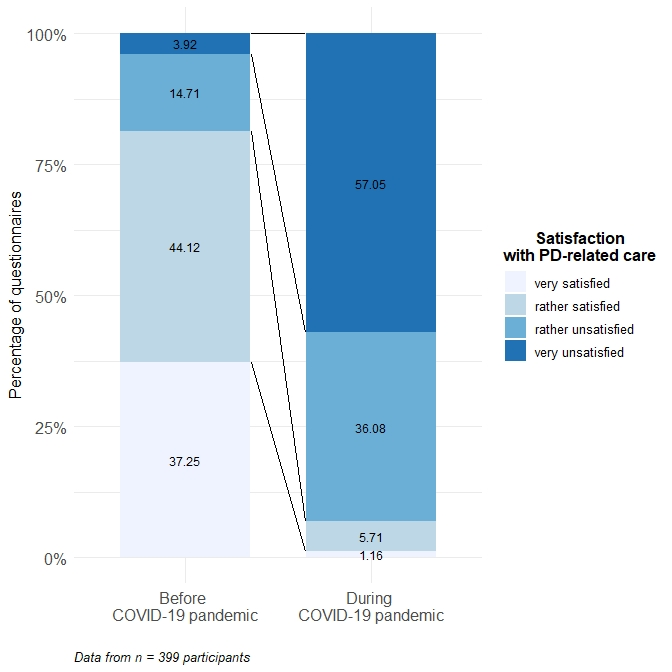
\includegraphics[width=.90\textwidth]{fig2.satisfaction.care.v1.0.jpeg}
\caption{Distribution of responses on the Satisfaction with PD-related care before and during the \textsc{Covid}-19 pandemic.}
\label{fig2:satisfaction}
\end{figure}

\begin{figure}
\centering
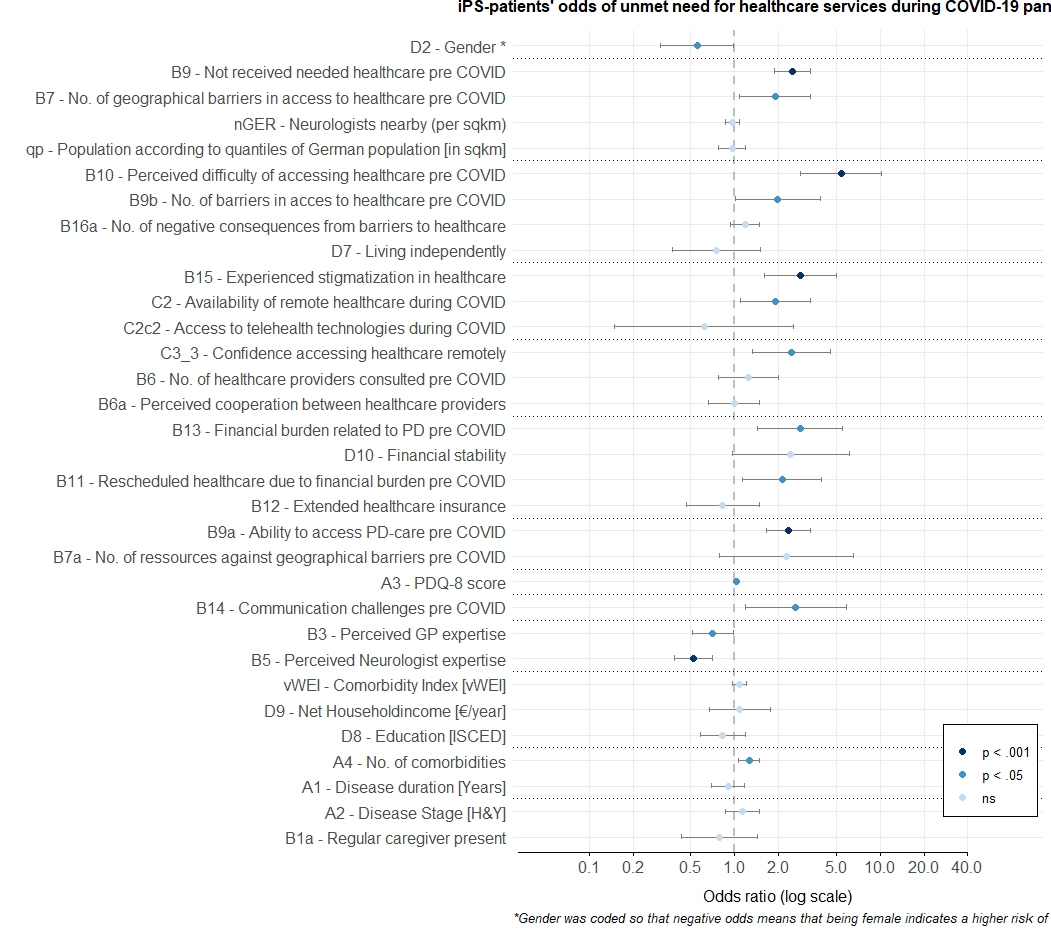
\includegraphics[width=.90\textwidth]{fig3.oddsratios.v1.0.jpeg}
\caption{Unadjusted Odds ratios according to the \ac{glm} for all 32 questions. Odds were determined so that higher values indicate affirmation to the question that healthcare was needed but this need remianed unmet during the \textsc{Covid}-19 pandemic. The dashed lines indicate the distinct domains according to ??, whereas significance is illustrated as color of the dot, with two distinct levels of significance. }%Quelle einfügen}
\label{fig3:resultsOR1}
\end{figure}




\newpage

	\section*{Discussion}
	Text for this section\ldots
	\section*{Conclusion}
	Text for this section\ldots
	\subsection*{Sub-heading for section}
	Text for this sub-heading\ldots
	\subsubsection*{Sub-sub heading for section}
	Text for this sub-sub-heading\ldots
	\paragraph*{Sub-sub-sub heading for section}
	Text for this sub-sub-sub-heading\ldots
	
	In this section we examine the growth rate of the mean of $Z_0$, $Z_1$ and $Z_2$. In
	addition, we examine a common modeling assumption and note the
	importance of considering the tails of the extinction time $T_x$ in
	studies of escape dynamics.
	We will first consider the expected resistant population at $vT_x$ for
	some $v>0$, (and temporarily assume $\alpha=0$)
	%
	\[
	E \bigl[Z_1(vT_x) \bigr]=
	\int_0^{v\wedge
		1}Z_0(uT_x)
	\exp (\lambda_1)\,du .
	\]
	%
	If we assume that sensitive cells follow a deterministic decay
	$Z_0(t)=xe^{\lambda_0 t}$ and approximate their extinction time as
	$T_x\approx-\frac{1}{\lambda_0}\log x$, then we can heuristically
	estimate the expected value as
	%
	\begin{equation}\label{eqexpmuts}
		\begin{aligned}[b]
			&      E\bigl[Z_1(vT_x)\bigr]\\
			&\quad      = \frac{\mu}{r}\log x
			\int_0^{v\wedge1}x^{1-u}x^{({\lambda_1}/{r})(v-u)}\,du .
		\end{aligned}
	\end{equation}
	%
	%Thus we observe that this expected value is finite for all $v>0$ (also see \cite{koon,xjon,marg,schn,koha,issnic}).
	
	
	\section*{Appendix}
	Text for this section\ldots
	
	%%%%%%%%%%%%%%%%%%%%%%%%%%%%%%%%%%%%%%%%%%%%%%
	%%                                          %%
	%% Backmatter begins here                   %%
	%%                                          %%
	%%%%%%%%%%%%%%%%%%%%%%%%%%%%%%%%%%%%%%%%%%%%%%
	
	\begin{backmatter}
		
		\section*{Acknowledgements}%% if any
		Text for this section\ldots
		
\section*{Funding}%% if any
This study was supported by the funds of the The EU Joint Programme – Neurodegenerative Disease Research (JPND).

D. P. received a grant from the German Research Foundation (PE 2291-1). D.P. received payments as a consultant for Boston Scientific and as a speaker at symposia sponsored by Boston Scientific and AbbVie. D.P.'s institution, not D.P. personally, received funding from the German Federal Joint Committee (G-BA), the German Federal Ministry of Education and Research, the Horizon 2020 program of the European Commission, Boston Scientific, the Parkinson’s Foundation, the Dr.-Reinfried Pohl Foundation, and the German Parkinson Association (dPV).
		
\section*{Abbreviations}
\begin{acronym}[ECU]
\acro{aic}[AIC]{Akaike Information Criterion}
\acro{dpv}[DPV]{Deutsche Parkinson Vereinigung}
\acro{glm}[GLM]{Generalised Linear Model}
\acro{gp}[GP]{General practitioner}
\acro{icarepd}[iCARE-PD]{abbreviation iCARE PD missing}
\acro{pd}[PD]{Parkinson's Disease}
\acro{pmm}[PMM]{Predictive Mean Matching Method}
\acro{sdh}[SDH]{Social determinants of health}
\end{acronym}		

\section*{Availability of data and materials}
Data from all participants and all analyses are available under \url{https://github.com/dpedrosac/covidPD}
		
		\section*{Ethics approval and consent to participate}%% if any
		Text for this section\ldots
		
		\section*{Competing interests}
		The authors declare that they have no competing interests.
		
		\section*{Consent for publication}%% if any
		Text for this section\ldots
		
		\section*{Authors' contributions}
		Text for this section \ldots
		
		\section*{Authors' information}%% if any
		Text for this section\ldots
		
		%%%%%%%%%%%%%%%%%%%%%%%%%%%%%%%%%%%%%%%%%%%%%%%%%%%%%%%%%%%%%
		%%                  The Bibliography                       %%
		%%                                                         %%
		%%  Bmc_mathpys.bst  will be used to                       %%
		%%  create a .BBL file for submission.                     %%
		%%  After submission of the .TEX file,                     %%
		%%  you will be prompted to submit your .BBL file.         %%
		%%                                                         %%
		%%                                                         %%
		%%  Note that the displayed Bibliography will not          %%
		%%  necessarily be rendered by Latex exactly as specified  %%
		%%  in the online Instructions for Authors.                %%
		%%                                                         %%
		%%%%%%%%%%%%%%%%%%%%%%%%%%%%%%%%%%%%%%%%%%%%%%%%%%%%%%%%%%%%%
		\section*{References}
		% if your bibliography is in bibtex format, use those command
		
		\bibliographystyle{vancouver} % Style BST file (bmc-mathphys, vancouver, spbasic).
		\bibliography{bmc_article_covidPD}      % Bibliography file (usually '*.bib' )
		
%%%%%%%%%%%%%%%%%%%%%%%%%%%%%%%%%%%
%%                               %%
%% Figures                       %%
%%                               %%
%% NB: this is for captions and  %%
%% Titles. All graphics must be  %%
%% submitted separately and NOT  %%
%% included in the Tex document  %%
%%                               %%
%%%%%%%%%%%%%%%%%%%%%%%%%%%%%%%%%%%
		
%%
%% Do not use \listoffigures as most will included as separate files
		
\newpage
\section*{Figures}
\begin{figure}[h!]
    \centering
    \begin{subfigure}[b]{0.35\linewidth}
        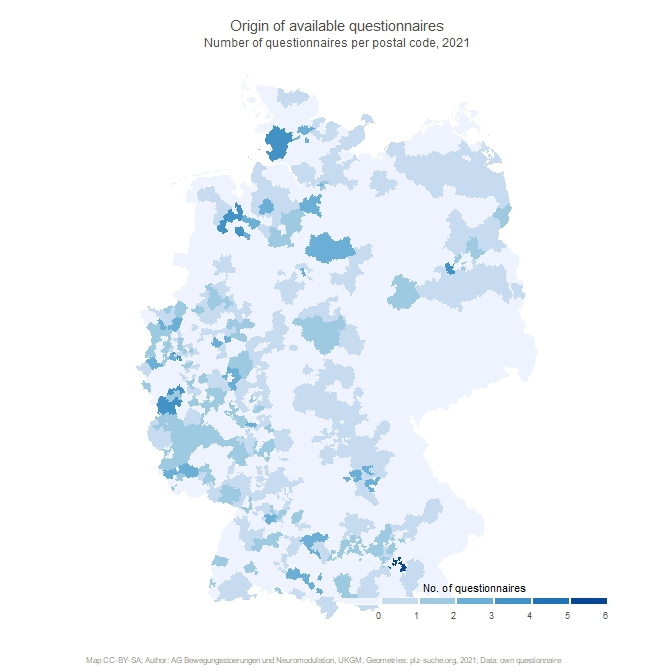
\includegraphics[width=.90\textwidth]{available.questionnaires.jpeg}
        \label{fig1:questionnaires}
    \end{subfigure}%
    \begin{subfigure}[b]{0.35\linewidth}
        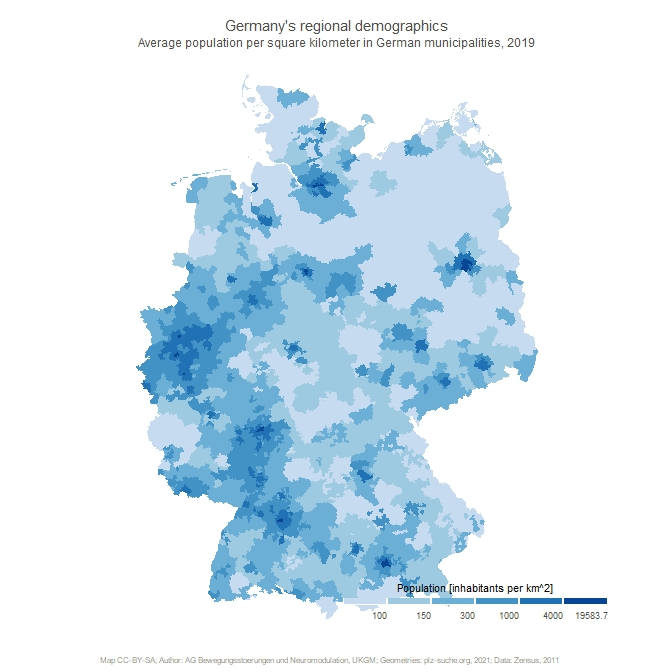
\includegraphics[width=.90\textwidth]{population.perskmGER.jpeg}
        \label{fig1:population}
    \end{subfigure}%
    \begin{subfigure}[b]{0.35\linewidth}
        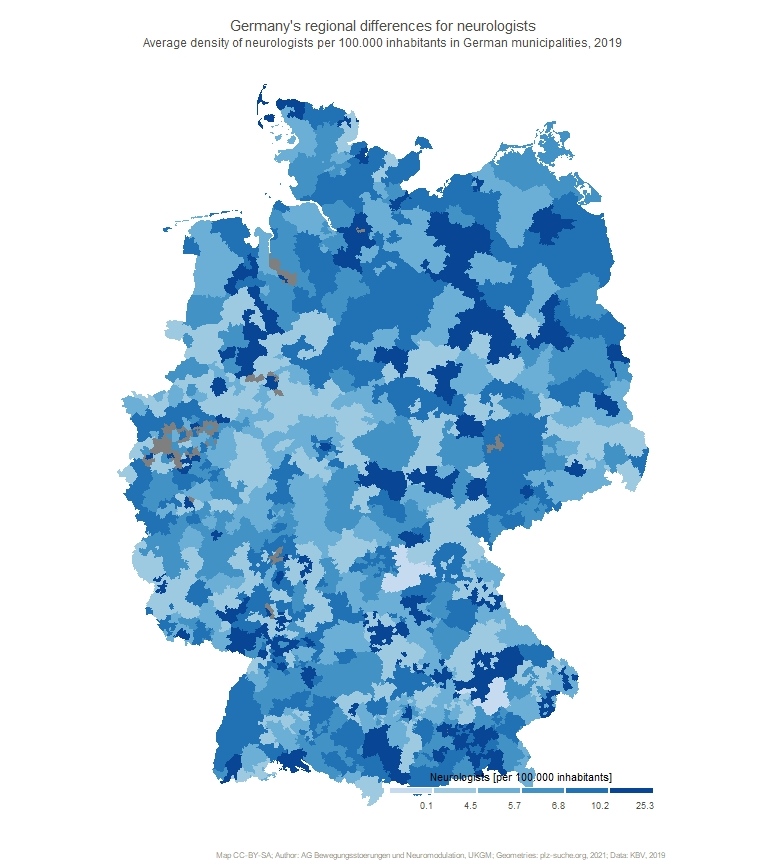
\includegraphics[width=.90\textwidth]{neurologists.10122021.jpeg}
        \label{fig1:neurologists}
    \end{subfigure}%
\caption{Demographic data for Germany and additional regional data for the obtained questionnaires. A) Number of received questionnaires within our survey for the distinct three digit postal codes. B) Illustration of inhabitants per square kilometer for Germany (source: \url{https://www.destatis.de}) C) Density of neurologists in all parts of Germany according to the German Statutory Health Insurance Association (Kassenärztliche Bundesvereinigung, \url{https://www.kbv.de/html/})}
\label{fig1:total}
\end{figure}
	
\newpage	
\begin{figure}[h!]
\includesvg[width=.84\textwidth]{fig2.satisfaction.care.v1.1}
\caption{Distribution of responses on the Satisfaction with PD-related care before and during the \textsc{Covid}-19 pandemic.}
\end{figure}

\newpage	
\begin{landscape}
\begin{figure}[h!]
\includesvg[width=.84\textwidth]{fig3.oddsratios.v1.1}
\caption{Logistic regression for distinct predictors. A \ac{glm} with a binomial logit function was used to estimate the odds for different questions and data from the questionnaires for affirding that ??. All odds are displayed on alogarithmic scale and significance level is color coded. For additional information cf. supplementary material.}
\end{figure}
\end{landscape}

\newpage
\begin{figure}[h!]
\includesvg[width=.84\textwidth]{fig4.model.comparison.v1.0}
\caption{Comparison of the models. The full model including all predictors was compatred in terms of accuracy to the reduced model resulting from the stepwise \ac{glm}regression. Values between both models are comparable although only ?? predictors remained in the model compared to the full model with ?? predictors. For further details of the multilevel regression cf. Table ??}
\end{figure}


%%%%%%%%%%%%%%%%%%%%%%%%%%%%%%%%%%%
%%                               %%
%% Tables                        %%
%%                               %%
%%%%%%%%%%%%%%%%%%%%%%%%%%%%%%%%%%%
		
\section*{Tables}
\begin{table}[!ht]
\begin{tabular}{p{5cm} c}
\toprule
																		&	\textbf{Overall}	\\ %\hline
																		& 	\textbf{(n = 552)}\\ 
\midrule
Age (mean (SD)) 															& 	66.76 (9.25) 	\\ \hline
Gender = female (\%) 														&  	148 (41.6)  		\\ \hline
Disease duration (\%) 														& 				\\ \hline
\hspace{3mm} $<$2 years 													& 	62 (13.1) 		\\ \hline
\hspace{3mm} 2--5 years 													& 	154 (32.6) 		\\ \hline
\hspace{3mm} 5--10 years 													& 	157 (33.2) 		\\ \hline
\hspace{3mm} 10--15 years 													& 	69 (14.6) 		\\ \hline
\hspace{3mm} $>$15 years													& 	31 ( 6.6) 		\\ \hline
Disease stage (\%)															& 				\\ \hline
\hspace{3mm} Hoehn \& Yahr I 												&  	189 (40.3) 		\\ \hline
\hspace{3mm} Hoehn \& Yahr II 												& 	156 (33.3)  		\\ \hline
\hspace{3mm} Hoehn \& Yahr III  												&   	77 (16.4) 		\\ \hline
\hspace{3mm} Hoehn \& Yahr IV  												& 	41 ( 8.7) 		\\ \hline
\hspace{3mm} Hoehn \& Yahr V  												&     	6 ( 1.3) 		\\ \hline
Education level according \newline to ISCED (\%) 									& 				\\ \hline
\hspace{3mm} primary education  												& 	20 ( 5.0) 		\\ \hline
\hspace{3mm} secondary education 						 					& 	234 (58.4)		\\ \hline
\hspace{3mm} post secondary education  										&   	69 (17.2) 		\\ \hline
\hspace{3mm} highest education level possible 										& 	78 (19.5)  		\\ \hline
\hspace{3mm} PDQ-8 scores (mean (SD)) 										& 	41.30 (14.23) 	\\ \hline
Van-Walraven-Elixhauser \newline \hspace{3mm} Comorbidity Index (mean (SD)) 	& 	6.55 (1.95) 		\\ 
\bottomrule
\caption{Demographics of subjects filling out questionnaire:}
\label{tab1:demographics}
\end{tabular}
\end{table}

\begin{table}[!ht]
    \centering
    \begin{tabular}{l l l l l}
    	\toprule    
        Predictor 												& Estimate 	& Std.Error & zvalue & \textit{p} \\
        \midrule
        (Intercept) 											&  -2.65  		& 0.29 	& -9.24 	& <.0001 \\ \hline
        Educational level (D8) 									& -0.73 		& 0.24 	& -3.01 	& 0.003 \\ \hline
        Perceived GP's expertise (B3) 							& 0.34" 		& 0.17 	& 2.07 	& 0.038 \\ \hline
        Confidence in accessing necessary services remotely (C3) 	& 0.64 		& 0.22 	& 2.90 	& 0.004 \\ \hline
        Ease obtaining healthcare prior to the pandemic (B10)		& -0.47 		& 0.22 	& -2.15 	& 0.031 \\ \hline
        Ability to access care prior to the pandemic (B9)				& 0.41 		& 0.20 	& 2.07 	& 0.038 \\ \hline
        Density of Neurologists 									& 0.47 		& 0.21 	& 2.22 	& 0.027 \\ \hline
        Overcoming barriers (B7a)   								& -0.51 		& 0.22 	& -2.38 	& 0.017 \\
        \bottomrule
    \end{tabular}
\caption{Significant factors contibuting to unmet care needs during \textsc{Covid}-19 pandemic according to the reduced \ac{glm}:}
\end{table}	

%%%%%%%%%%%%%%%%%%%%%%%%%%%%%%%%%%%
%%                               %%
%% Additional Files              %%
%%                               %%
%%%%%%%%%%%%%%%%%%%%%%%%%%%%%%%%%%%
		
\section*{Additional Files}
\begin{table}[!ht]
    \centering
    \begin{tabular}{l l}
    \toprule
        \textbf{Question from COVID Survey}	& \textbf{Representative for what barrierer} \\
	\midrule
        1. A2, B1 							& Autonomy \\ \hline
        2. A1, A4, vWEI 					& Health Status \\ \hline
        3. D8, D9 							& Health Literacy \\ \hline
        4. B3, B5 							& Health Belief \\ \hline
        5. B14a 							& Communication (personal) \\ \hline
        6. PDQ-sum score 					& Self-efficacy \\ \hline
        7. B7a, B9a/b 						& Transportation \\ \hline
        8. B11, B12, B13, D10 				& Cost of care \\ \hline
        9. NA 							& Difficulties of Diagnosis \\ \hline
        10. C3, B6a, B6 					& Coordination in care \\ \hline
        11. B15, B14, C2c 					& Communication (system) \\ \hline
        12. B16, B16c, D6, D7, B9b, B10 		& Disparty in Health Services \\ \hline
        13. B7, B8, B9, 						& Unavailability of Specalist Services \\ \hline
        14. D2 							& Other \\
        \bottomrule
    \end{tabular}
\caption{Matching of items in the questionnaire to the categories from the work of Zaman et al. \cite{zaman2021barriers}}
\end{table}

\begin{table}[!ht]
    \centering
    \begin{tabular}{|l|l|l|l|l|l|}
    \hline
        "Factors" & "Domain" & "Odds Ratio" & "CI.05" & "CI.95" & "p-value" \\ \hline
        "A2 - Disease Stage [H\&Y]" & "Autonomy" & 1.13 & 0.87 & 1.47 & "0.367" \\ \hline
        "B1a - Regular caregiver present" & "Autonomy" & 0.79 & 0.43 & 1.44 & "0.438" \\ \hline
        "A1 - Disease duration [Years]" & "Health Status" & 0.9 & 0.69 & 1.16 & "0.419" \\ \hline
        "A4 - No. of comorbidities" & "Health Status" & 1.26 & 1.06 & 1.49 & "0.007" \\ \hline
        "vWEI - Comorbidity Index [vWEI]" & "Health Belief" & 1.08 & 0.97 & 1.21 & "0.155" \\ \hline
        "D8 - Education [ISCED]" & "Health Belief" & 0.82 & 0.58 & 1.18 & "0.284" \\ \hline
        "D9 - Net Householdincome [per/year]" & "Health Belief" & 1.08 & 0.67 & 1.75 & "0.75" \\ \hline
        "B3 - Perceived GP expertise" & "Health Literacy" & 0.71 & 0.51 & 0.98 & "0.038" \\ \hline
        "B5 - Perceived Neurologist expertise" & "Health Literacy" & 0.52 & 0.39 & 0.7 & "p < .001" \\ \hline
        "B14 - Communication challenges pre COVID" & "Communication (personal)" & 2.63 & 1.18 & 5.82 & "0.017" \\ \hline
        "A3 - PDQ-8 score" & "Self-efficacy" & 1.03 & 1.01 & 1.05 & "0.011" \\ \hline
        "B7a - No. of ressources against geographical barriers pre COVID" & "Transportation" & 2.27 & 0.79 & 6.51 & "0.129" \\ \hline
        "B9a - Ability to access PD-care pre COVID" & "Transportation" & 2.33 & 1.65 & 3.31 & "p < .001" \\ \hline
        "B11 - Rescheduled healthcare due to financial burden pre COVID" & "Cost of care" & 2.11 & 1.13 & 3.93 & "0.019" \\ \hline
        "B12 - Extended healthcare insurance" & "Cost of care" & 0.83 & 0.46 & 1.48 & "0.521" \\ \hline
        "B13 - Financial burden related to PD pre COVID" & "Cost of care" & 2.81 & 1.42 & 5.53 & "0.003" \\ \hline
        "D10 - Financial stability" & "Cost of care" & 2.43 & 0.97 & 6.09 & "0.059" \\ \hline
        "C3\_3 - Confidence accessing healthcare remotely" & "Difficulties of Diagnosis" & 2.44 & 1.32 & 4.53 & "0.005" \\ \hline
        "B6a - Perceived cooperation between healthcare providers" & "Difficulties of Diagnosis" & 0.99 & 0.66 & 1.49 & "0.975" \\ \hline
        "B6 - No. of healthcare providers consulted pre COVID" & "Difficulties of Diagnosis" & 1.24 & 0.77 & 1.99 & "0.374" \\ \hline
        "B15 - Experienced stigmatization in healthcare" & "Coordination in care" & 2.84 & 1.6 & 5.03 & "p < .001" \\ \hline
        "C2 - Availability of remote healthcare during COVID" & "Coordination in care" & 1.91 & 1.09 & 3.34 & "0.023" \\ \hline
        "C2c2 - Access to telehealth technologies during COVID" & "Coordination in care" & 0.62 & 0.15 & 2.53 & "0.5" \\ \hline
        "B16a - No. of negative consequences from barriers to healthcare" & "Communication (system)" & 1.18 & 0.93 & 1.48 & "0.166" \\ \hline
        "D7 - Living independently" & "Communication (system)" & 0.75 & 0.38 & 1.51 & "0.421" \\ \hline
        "B9b - No. of barriers in acces to healthcare pre COVID" & "Communication (system)" & 1.98 & 1.01 & 3.89 & "0.048" \\ \hline
        "B10 - Perceived difficulty of accessing healthcare pre COVID" & "Communication (system)" & 5.37 & 2.84 & 10.17 & "p < .001" \\ \hline
        "B7 - No. of geographical barriers in access to healthcare pre COVID" & "Disparty in Health Services" & 1.9 & 1.08 & 3.33 & "0.026" \\ \hline
        "  Population according to quantiles of German population [in sqkm]" & "Disparty in Health Services" & 0.96 & 0.77 & 1.19 & "0.714" \\ \hline
        "B9 - Not received needed healthcare pre COVID" & "Disparty in Health Services" & 2.5 & 1.88 & 3.32 & "p < .001" \\ \hline
        "nGER - Neurologists nearby (per sqkm)" & "Disparty in Health Services" & 0.97 & 0.87 & 1.07 & "0.527" \\ \hline
        "D2 - Gender *" & "Unavailability of Specalist Services" & 0.55 & 0.31 & 0.98 & "0.044" \\ \hline
    \end{tabular}
\caption{Odds ratios for the distinct items of the questionnaire}

\end{table}

\subsection*{Additional file 1 --- Sample additional file title}
Additional file descriptions text (including details of how to
view the file, if it is in a non-standard format or the file extension).  This might
refer to a multi-page table or a figure.

		
\subsection*{Additional file 2 --- Sample additional file title}
Additional file descriptions text.
\end{backmatter}
\end{document}
